% IC2E 2026 short-paper working copy.
% Keep the main draft in calibration_aware_autoscaling_paper.tex unchanged.
\documentclass[11pt]{article}
\usepackage[margin=1in]{geometry}
\usepackage[T1]{fontenc}
\usepackage[utf8]{inputenc}
\usepackage{lmodern}
\usepackage{amsmath,amssymb,amsthm}
\usepackage{booktabs}
\usepackage{graphicx}
\usepackage{hyperref}
\usepackage{xcolor}
\usepackage{enumitem}
\usepackage{microtype}

\theoremstyle{plain}
\newtheorem{theorem}{Theorem}[section]
\newtheorem{proposition}[theorem]{Proposition}
\newtheorem{lemma}[theorem]{Lemma}
\theoremstyle{definition}
\newtheorem{definition}[theorem]{Definition}
\newtheorem{assumption}[theorem]{Assumption}
\theoremstyle{remark}
\newtheorem{remark}[theorem]{Remark}

\hypersetup{
  colorlinks=true,
  linkcolor=blue,
  citecolor=blue,
  urlcolor=blue
}

\title{When Forecast Accuracy Is Not Enough:\\Calibration-Aware Autoscaling for Bursty Serverless Workloads (Short Paper)}
\author{Dang Le}
\date{\today}

\begin{document}
\maketitle

\begin{abstract}
Reactive autoscaling responds too late to sudden demand spikes, while point-forecast policies ignore uncertainty and can underprovision under bursty workloads. This paper studies autoscaling as a decision problem under predictive uncertainty and asks whether calibration quality, not only point accuracy, changes downstream scaling quality. We propose a lightweight calibration-aware policy that uses residual-calibrated demand scenarios inside an explicit cost-reliability objective. On the public Azure Functions Invocation Trace 2021, predictive methods reduce aggregate SLA violations substantially relative to reactive scaling, but burst-only evaluation shows that all current methods remain fragile on rare spikes. The main contribution of the paper is therefore not a final controller, but a reproducible empirical and theoretical case that calibration-aware evaluation exposes failure modes that average metrics can hide.
\end{abstract}

\section{Introduction}
Cloud autoscaling is fundamentally a decision-making problem under uncertainty. In practice, many policies are either reactive, triggered by observed threshold violations, or predictive, driven by point forecasts of near-term demand. Both paradigms are brittle under bursty workloads: reactive rules respond too late, while point forecasts hide uncertainty and encourage unsafe capacity decisions.

This short paper asks a narrower question than a full controller paper: \emph{does calibration quality materially affect downstream autoscaling quality?} Our hypothesis is that forecast accuracy alone is not enough. A forecaster can have small average error yet still produce badly miscalibrated upper tails, and those tail errors translate directly into underprovision events.

We study this question on the public Azure Functions Invocation Trace 2021. The paper makes three contributions. First, it formulates autoscaling as a calibration-sensitive decision problem and gives a simple theorem linking calibrated upper bounds to SLA control. Second, it instantiates this idea with a lightweight residual-calibrated scaling policy that is easy to reproduce on a public serverless trace. Third, it shows empirically that burst-only evaluation reveals failures that aggregate metrics hide, including for calibration-aware methods.

\section{Related Work}
Predictive autoscaling has been studied through workload forecasting, control-oriented provisioning, and learning-based controllers \cite{roy2011efficient,gandhi2014adaptive,qiu2023aware}. A separate line of work studies predictive calibration and interval validity \cite{guo2017calibration,shafer2008tutorial,xu2021conformal}. Our paper sits between these two threads. Rather than proposing a richer controller stack or a full conformalized method, it asks a simpler systems question: when autoscaling decisions depend on upper-tail demand estimates, how much does calibration quality matter, and what do burst-only evaluations reveal that average metrics miss?

\section{Problem Formulation and Theoretical Motivation}
Let $H_t$ denote the observed application-level workload history up to time $t$, and let $D_{t+h} \in \mathbb{Z}_{\ge 0}$ denote the random required capacity at forecast horizon $h$. The autoscaling decision is to choose an integer capacity $c_t \in \mathbb{Z}_{\ge 0}$ before $D_{t+h}$ is observed.

The paper treats autoscaling as a decision problem under predictive uncertainty. For history $H_t$ and future required capacity $D_{t+h}$, the policy chooses capacity $c_t$ by minimizing
\[
\mathcal{L}_t(c_t) =
\lambda_c \, c_t
\;+\;
\lambda_u \, \mathbb{E}\!\left[(D_{t+h} - c_t)_+\right]
\;+\;
\lambda_s \, |c_t - c_{t-1}|,
\]
where $(x)_+ = \max(x,0)$, $\lambda_c > 0$ is the unit provisioning cost, $\lambda_u > 0$ is the underprovision penalty weight, and $\lambda_s > 0$ penalizes oscillatory scaling.

This objective is intentionally simple: it connects predictive uncertainty to downstream decisions while remaining interpretable and easy to evaluate on a public trace.

When $\lambda_s=0$ and the demand distribution is known exactly, the optimizer of the asymmetric-cost objective reduces to a demand quantile. This gives a clean interpretation of fixed-quantile scaling: it is a simplified decision rule under known uncertainty, not an arbitrary heuristic.

\begin{theorem}[Calibration transfers directly to SLA control]
\label{thm:calibration-to-sla}
Let $U_{1-\alpha}(H_t)$ satisfy
\[
\mathbb{P}\!\bigl(D_{t+h} \le U_{1-\alpha}(H_t)\bigr) \ge 1-\alpha-\varepsilon.
\]
If the policy chooses
\[
c_t = \left\lceil U_{1-\alpha}(H_t) \right\rceil,
\]
then
\[
\mathbb{P}(D_{t+h} > c_t) \le \alpha + \varepsilon.
\]
\end{theorem}
\begin{proof}[Proof sketch]
Because $c_t \ge U_{1-\alpha}(H_t)$ by construction,
\[
\{D_{t+h} > c_t\} \subseteq \{D_{t+h} > U_{1-\alpha}(H_t)\}.
\]
Taking probabilities and using $\varepsilon$-upper-calibration gives
\[
\mathbb{P}(D_{t+h} > c_t)
\le
1 - \mathbb{P}\!\bigl(D_{t+h} \le U_{1-\alpha}(H_t)\bigr)
\le
\alpha + \varepsilon.
\]
\end{proof}

Theorem~\ref{thm:calibration-to-sla} is the core reason the paper cares about calibration. A nominal ``P95'' autoscaling rule only deserves that interpretation if the deployed upper bound is close to a true 95th percentile. The current implementation uses empirical residual quantiles rather than a full conformalized construction, so the paper does not claim an exact finite-sample guarantee.

\section{Method}
\label{sec:method}
\subsection{Forecasting Model}
For each application we construct a minute-level required-capacity sequence $\{y_t\}_{t=1}^T$. Given a history window of length $m$ and forecast horizon $h$, the forecasting module predicts
\[
\hat y_{t+h} = f_{\theta}(y_{t-m+1}, \ldots, y_t).
\]
In the current implementation, $f_\theta$ is a linear autoregressive model. This choice is deliberate: it keeps the predictor simple enough that downstream differences can be attributed mainly to calibration and decision logic rather than to model scale.

\subsection{Calibration Layer}
Let $\mathcal{I}_{\mathrm{cal}}$ denote the calibration split and define residuals
\[
r_i = y_i - \hat y_i, \qquad i \in \mathcal{I}_{\mathrm{cal}}.
\]
The method uses the empirical residual distribution in two ways. First, it forms a calibrated interval
\[
\bigl[\ell_{t+h}, u_{t+h}\bigr]
=
\Bigl[
\max(0,\hat y_{t+h}+q_{\alpha/2}(R)),
\max(0,\hat y_{t+h}+q_{1-\alpha/2}(R))
\Bigr],
\]
where $R=\{r_i : i\in\mathcal{I}_{\mathrm{cal}}\}$ and $q_p(R)$ denotes the empirical $p$-quantile of the residual set. Second, it forms a scenario set for downstream decisions,
\[
\mathcal{S}_{t+h} = \{\max(\hat y_{t+h}+r,0): r \in R\}.
\]
The default configuration pools residuals globally.

\subsection{Decision Layer}
Given the scenario set $\mathcal{S}_{t+h}$ and previous capacity $c_{t-1}$, the calibration-aware policy chooses
\[
\hat c_t
=
\arg\min_{c \in \mathbb{Z}_{\ge 0}}
\left[
\lambda_c c
\;+\;
\lambda_u \frac{1}{|\mathcal{S}_{t+h}|} \sum_{s \in \mathcal{S}_{t+h}} (s-c)_+
\;+\;
\lambda_s |c-c_{t-1}|
\right].
\]
This objective balances provisioning cost, expected underprovision under calibrated demand scenarios, and temporal smoothness. The candidate set is discrete, so the implementation solves the objective by enumeration over a bounded integer range.

\section{Experimental Setup}
The empirical study uses the Azure Functions Invocation Trace 2021 as a public serverless case study. For each invocation, start time is reconstructed from the released end timestamp and duration, after which the trace is aggregated at the application level into 1-minute buckets. The main target is minute-level required capacity derived from average concurrent demand within each minute. The primary setup keeps the top 10 most active applications, uses chronological train/validation/test splits of 70/15/15, and evaluates a 5-minute forecast horizon.

We compare the proposed method against four baselines: reactive threshold autoscaling, moving-average forecasting, linear autoregressive point forecasting, and fixed-quantile scaling at level $0.95$. The main downstream metrics are mean provisioning cost, SLA violation rate, and oscillation. To expose rare-spike behavior, we report both aggregate test-set results and burst-only results obtained from a rolling-baseline burst detector.

\section{Results}
The current codebase has been executed end-to-end under the setup described above. The results should be interpreted as a first full empirical pass on the public trace rather than as the final optimized version of the method.

\subsection{Aggregate Comparison}
Table~\ref{tab:aggregate-results} summarizes the first aggregate comparison on the test split.

\begin{table}[h]
\centering
\caption{Preliminary aggregate comparison on the Azure Functions 2021 test split. Lower is better for cost, SLA violation, and oscillation.}
\label{tab:aggregate-results}
\begin{tabular}{lccc}
\toprule
Method & Mean Cost & SLA Violation Rate & Mean Oscillation \\
\midrule
Reactive & 0.626 & 0.0318 & 0.1566 \\
Moving average & 0.543 & 0.0197 & 0.0225 \\
Point forecast & 1.044 & 0.0114 & 0.0754 \\
Fixed quantile (0.95) & 1.067 & 0.0205 & 0.0480 \\
Risk-calibrated & 1.038 & 0.0115 & 0.0678 \\
\bottomrule
\end{tabular}
\end{table}

Two observations already stand out. First, reactive scaling is clearly inferior on aggregate reliability: its SLA violation rate is roughly three times that of the point-forecast and calibration-aware methods. Second, the risk-calibrated policy is competitive with the point-forecast baseline on aggregate performance, yielding slightly lower mean cost and lower oscillation, but not yet a decisive SLA improvement.

\subsection{Burst-Only Evaluation}
Aggregate performance is not the full story. We therefore isolate burst windows using a rolling-baseline detector and compare methods only on those windows. In the current test split, burst windows make up only about $1.23\%$ of all decision steps, but they are much harder than the average case.

\begin{table}[h]
\centering
\caption{Preliminary burst-only comparison. Lower is better for cost, SLA violation, and oscillation.}
\label{tab:burst-results}
\begin{tabular}{lccc}
\toprule
Method & Mean Cost & SLA Violation Rate & Mean Oscillation \\
\midrule
Reactive & 4.881 & 0.7665 & 3.4229 \\
Moving average & 0.546 & 0.9604 & 0.0617 \\
Point forecast & 1.013 & 0.7885 & 0.0396 \\
Fixed quantile (0.95) & 0.925 & 0.9207 & 0.0044 \\
Risk-calibrated & 1.009 & 0.7885 & 0.0352 \\
\bottomrule
\end{tabular}
\end{table}

These results sharpen the paper's motivation. All current methods still fail badly on burst windows, including the calibration-aware one. However, they fail in different ways: reactive scaling becomes extremely expensive and unstable, while smoothing and fixed-quantile policies remain cheap but miss bursts almost completely. The point-forecast and risk-calibrated policies are the strongest among the current methods on burst windows, yet their SLA violation rates remain far too high. This suggests that the main research opportunity lies not in squeezing small gains from average-case metrics, but in improving burst sensitivity without giving up reproducibility.

Figure~\ref{fig:burst-case-study} makes this failure mode concrete on a representative episode selected automatically from the test split as the burst with the largest total underprovision under the current risk-calibrated policy. Reactive scaling chases the spike only after it arrives, producing large oscillations. The point-forecast and risk-calibrated policies are noticeably smoother, but both still lag the burst peak. The risk-calibrated interval widens around the event, yet not enough to cover the sharpest jump. This is exactly the paper's current empirical takeaway: calibration helps structure the decision problem, but burst robustness still requires a stronger decision rule or a more burst-sensitive uncertainty model.

\begin{figure}[h]
\centering
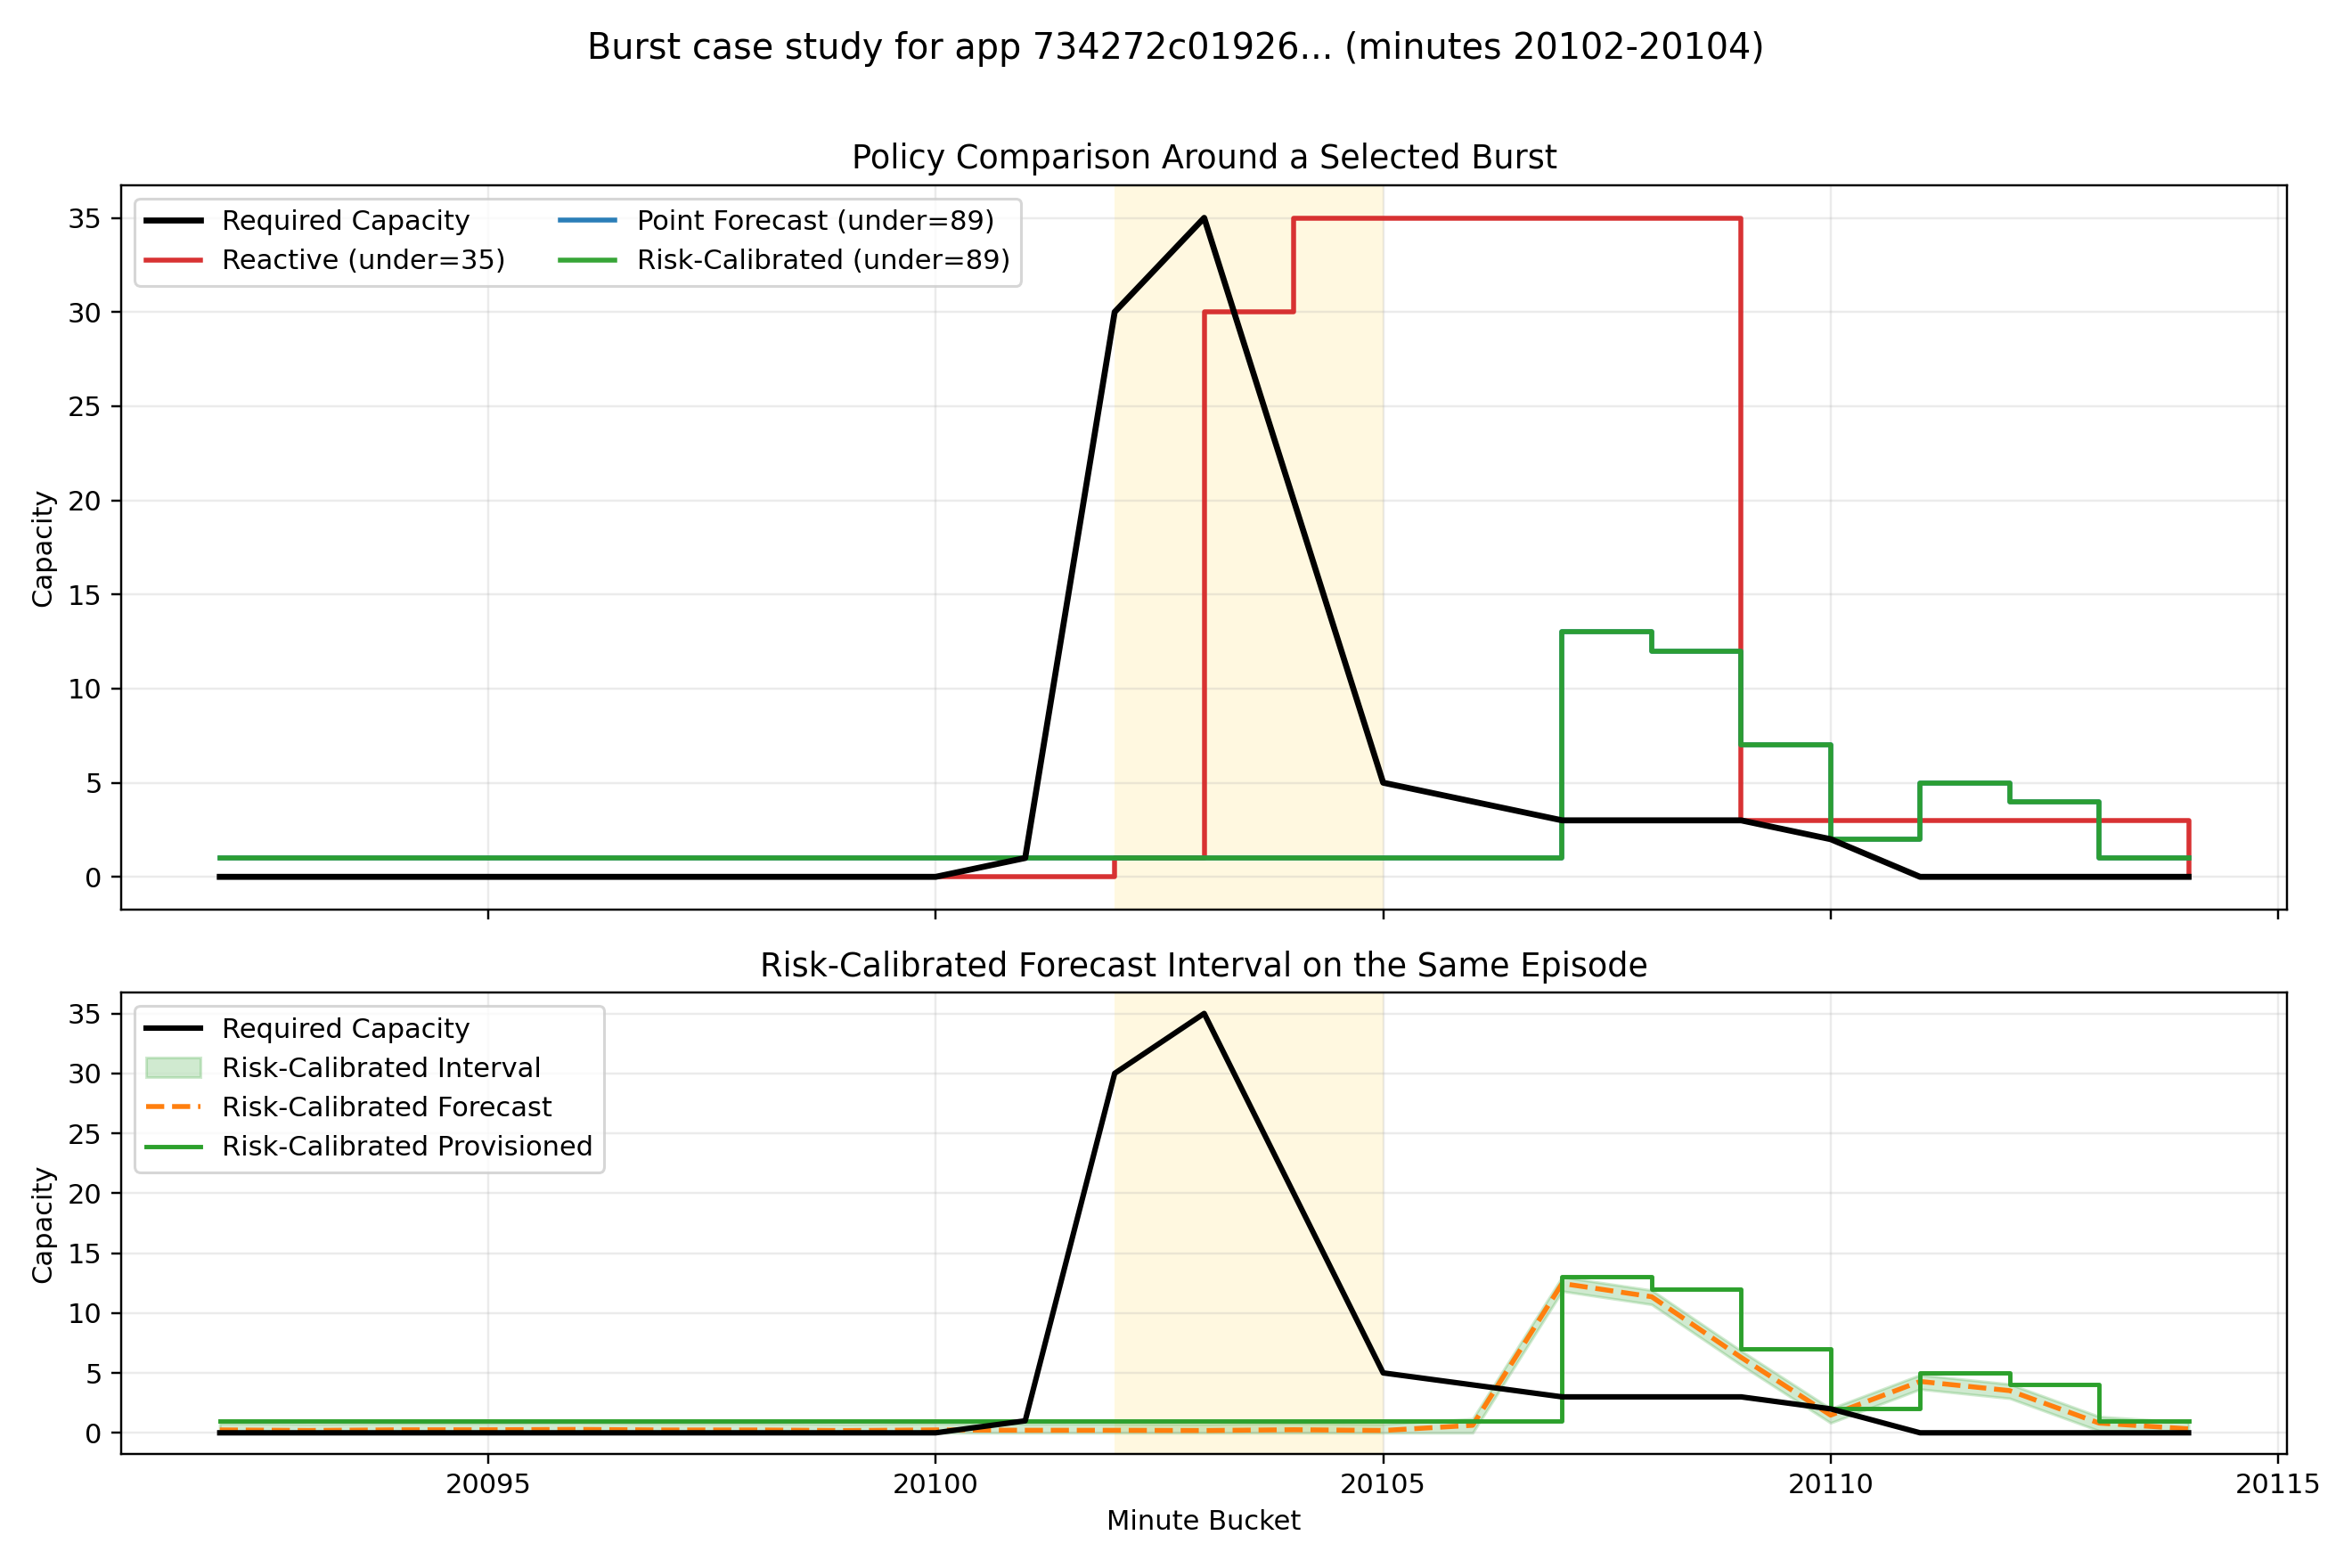
\includegraphics[width=\linewidth]{figures/burst_case_study.png}
\caption{Burst case study selected automatically from the test split. The top panel compares realized required capacity against the provisioned capacity chosen by reactive, point-forecast, and risk-calibrated policies. The bottom panel shows the risk-calibrated forecast interval over the same window. All three policies underreact to the sharp spike, but reactive scaling does so with much higher oscillation.}
\label{fig:burst-case-study}
\end{figure}

For the risk-calibrated implementation with nominal coverage $0.90$, the empirical coverage on the test split is $0.8793$, giving a calibration gap of $0.0207$. This is close enough to make calibration decision-relevant, but not close enough to solve burst robustness on its own.

\section{Limitations and Future Work}
The current calibration layer is residual-based rather than fully conformalized, so the paper argues from population-level calibration logic rather than exact finite-sample guarantees. The empirical study also uses one public serverless trace and one primary capacity proxy, so the results should be read as a focused first case study rather than a broad claim across cloud settings. Future work should prioritize burst-sensitive decision logic before larger forecasting models.

\section{Conclusion}
This paper studies autoscaling as a risk-sensitive decision problem rather than a pure forecasting problem. The theory section shows why calibration error translates directly into SLA error, and the empirical study shows that average-case forecasting accuracy alone is not enough to characterize scaling quality. On the Azure Functions 2021 trace, calibration-aware scaling is competitive on aggregate metrics, while burst-only evaluation shows that average metrics understate the difficulty of rare demand spikes. Taken together, these results support the paper's central claim: predictive uncertainty is useful for autoscaling only when it is calibrated and coupled to an appropriate decision rule.

\begin{thebibliography}{99}
\bibitem{roy2011efficient}
Nilabja Roy, Abhishek Dubey, and Aniruddha S. Gokhale.
\newblock Efficient autoscaling in the cloud using predictive models for workload forecasting.
\newblock In {\em 2011 IEEE 4th International Conference on Cloud Computing (CLOUD)}, pages 500--507, 2011.

\bibitem{gandhi2014adaptive}
Anshul Gandhi, Parijat Dube, Alexei Karve, Andrzej Kochut, and Li Zhang.
\newblock Adaptive, model-driven autoscaling for cloud applications.
\newblock In {\em 11th International Conference on Autonomic Computing (ICAC 14)}, pages 57--64, 2014.

\bibitem{qiu2023aware}
Haoran Qiu, Weichao Mao, Chen Wang, Hubertus Franke, Alaa Youssef, Zbigniew T. Kalbarczyk, Tamer Basar, and Ravishankar K. Iyer.
\newblock {AWARE}: Automate workload autoscaling with reinforcement learning in production cloud systems.
\newblock In {\em 2023 USENIX Annual Technical Conference (USENIX ATC 23)}, pages 387--402, 2023.

\bibitem{guo2017calibration}
Chuan Guo, Geoff Pleiss, Yu Sun, and Kilian Q. Weinberger.
\newblock On calibration of modern neural networks.
\newblock In {\em Proceedings of the 34th International Conference on Machine Learning}, volume 70 of {\em Proceedings of Machine Learning Research}, pages 1321--1330, 2017.

\bibitem{shafer2008tutorial}
Glenn Shafer and Vladimir Vovk.
\newblock A tutorial on conformal prediction.
\newblock {\em Journal of Machine Learning Research}, 9:371--421, 2008.

\bibitem{xu2021conformal}
Chen Xu and Yao Xie.
\newblock Conformal prediction interval for dynamic time-series.
\newblock In {\em Proceedings of the 38th International Conference on Machine Learning}, volume 139 of {\em Proceedings of Machine Learning Research}, pages 11559--11569, 2021.
\end{thebibliography}

\end{document}
